\section{Results}
\subsection{Result from tracking}

How well it tracked objects and how many it could track at the same time.

\subsection{Analysing training different configurations and their charts}

Different model configuration and the test results. Charts of accuracy and loss.

\subsection{Results from doing object detection in matlab}
A Matlab script was tried in order to find possible ways of segmenting out regions containing objects in an image. The output segments would then each be classified separately. This way we would have both object locations and classifications on each object. \ref{fig:matlabImages} shows an example of this. However, results from this were highly unpredictable and the parameters were too dependent on lighting, shadows, the background among other features. Hence, this method was scrapped.

\subsection{Results from doing object detection with Turi}
Because of the vast amount of possible use cases it was decided to scale the objective down. The model was trained only on a few floor backgrounds. 

The mean average precision from the different models that were trained were observed and can be read in table \ref{table:mAP}. 

WE SHOULD PUT NUMBER OF IMAGES INSTEAD OF A PERCENTAGE

\begin{table}[h]
\centering
\begin{tabular}{ |c|c|c| } 
 \hline
 Amount of training images & Percentage of total amount & mean\_average\_precision  \\ 
 \hline
 $\approx 50$& 5\% & 0.17064 \\
 \hline
 $\approx 185$& 20\% & 0.39269 \\
 \hline
 $\approx 370$& 40\% & 0.40595 \\
 \hline
 $\approx 450$& 50\% & 0.47397 \\
 \hline
 $\approx 700$& 75\% & 0.54433 \\
 \hline
\end{tabular}
\caption{Mean average precision depending on the amount of training data used. 100\% corresponds to 926 images. HOW MANY IMAGES WERE TESTED ON? HOW WAS THE TEST CONDUCTED?}
\label{table:mAP}
\end{table}

These values can then be plotted giving us the graph shown in figure \ref{fig:mAPResult}

[SAMPLE BILD TILLS VI HAR GENERERAT KORREKT PLOT]
\begin{figure}[h]
\begin{center}
\includegraphics[width = 0.2\textwidth]{./Images/3dscanning1.png}
\caption{Mean Average Precision plotted against the amount of training data used. 100\% corresponds to 926 images.}
\label{fig:mAPResult}
\end{center}
\end{figure}

[iNCLUDE IMAGES FROM TESTING  IN TURI]


\subsection{Overall performance of the app}
%Something something what


\subsection{User tests}

A user survey was done in order to evaluate the performance of the application. By having a multitude of interested people booking time slots for a ten minute testing period, a decent amount of sample data could be gathered and evaluated. Figures \ref{fig:question1} to \ref{fig:question6} show bar charts and pie charts representing the answers gathered from the participants to some of the questions they were asked. 

\begin{figure}[hbtp]
\begin{center}
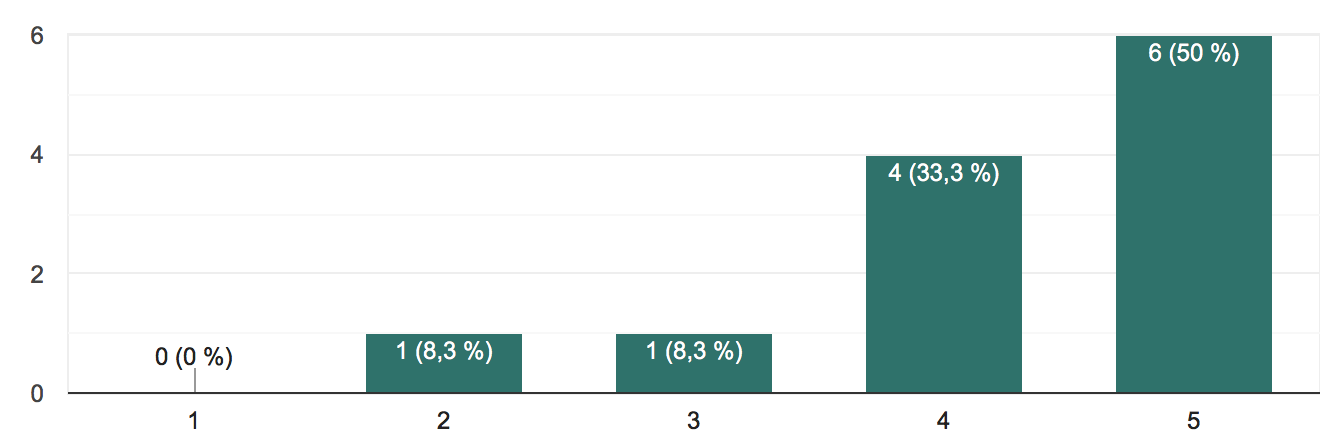
\includegraphics[width = 0.9\textwidth]{./Images/easyToGetToNext.png}
\caption{Results from when users were asked "How easy was it to understand how to get to the next step?"}
\label{fig:question1}
\end{center}
\end{figure}

\begin{figure}[hbtp]
\begin{center}
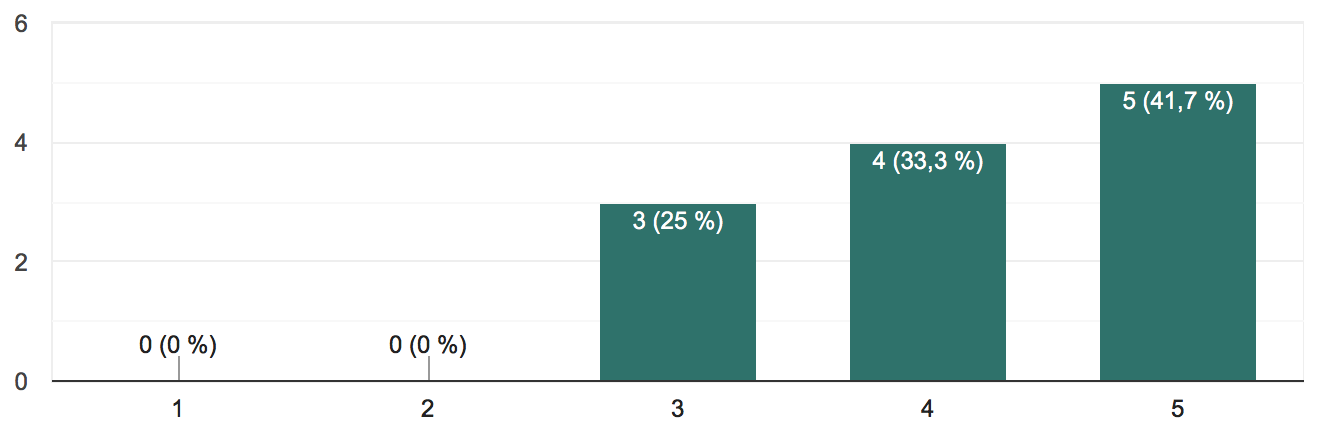
\includegraphics[width = 0.9\textwidth]{./Images/easyToUnderstand.png}
\caption{Results from when users were asked "How easy was it to understand how the pieces fit together?"}
\label{fig:question2}
\end{center}
\end{figure}

\begin{figure}[hbtp]
\begin{center}
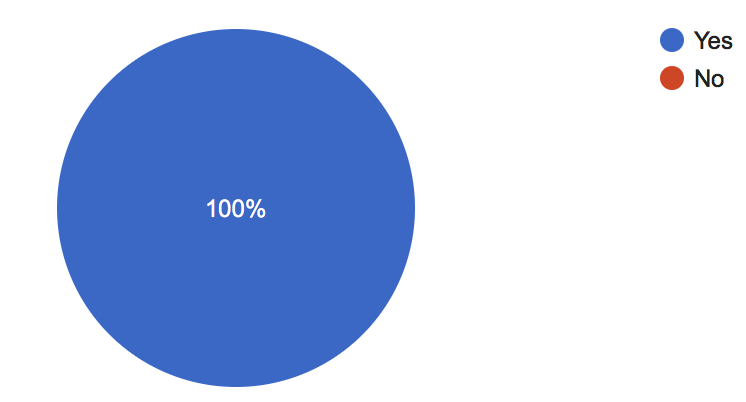
\includegraphics[width = 0.6\textwidth]{./Images/knowToSkip.png}
\caption{Results from when users were asked "Did you know that you could skip instructions?"}
\label{fig:question3}
\end{center}
\end{figure}

\begin{figure}[hbtp]
\begin{center}
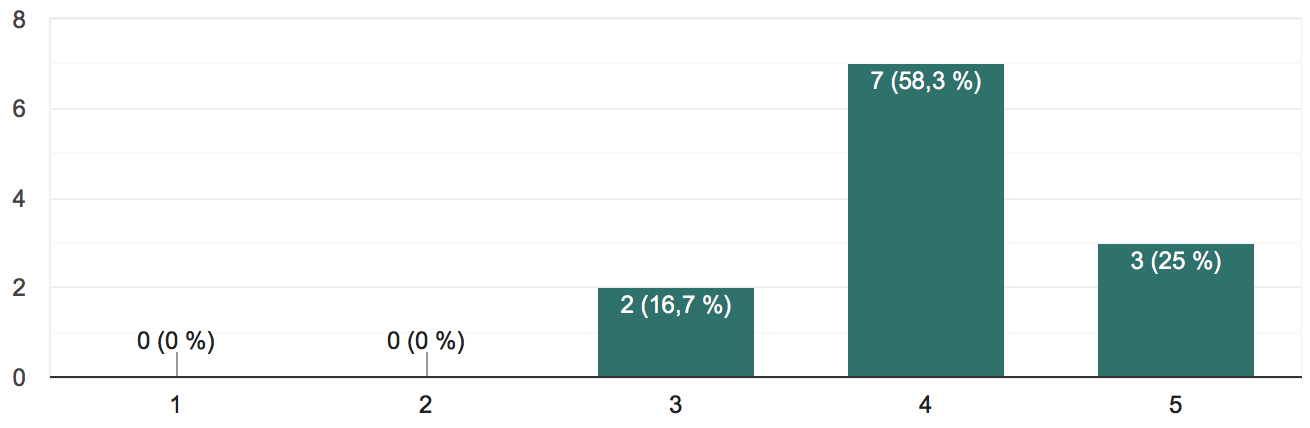
\includegraphics[width = 0.9\textwidth]{./Images/easyToUse.png}
\caption{Results from when users were asked "How easy was it to understand how to get to the next step?"}
\label{fig:question4}
\end{center}
\end{figure}

\begin{figure}[hbtp]
\begin{center}
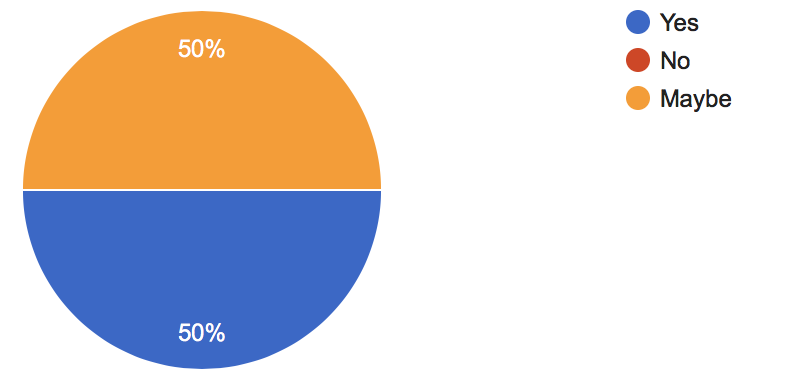
\includegraphics[width = 0.6\textwidth]{./Images/comparedTo.png}
\caption{Results from when users were asked "Compared to using paper instructions, did the app make it easier to understand how to put together the furniture?"}
\label{fig:question5}
\end{center}
\end{figure}

\begin{figure}[hbtp]
\begin{center}
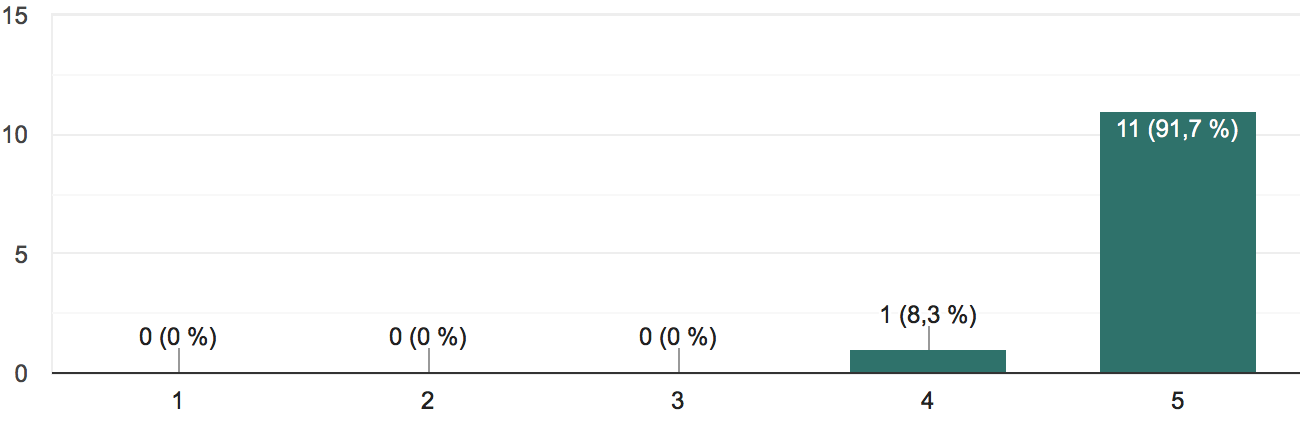
\includegraphics[width = 0.9\textwidth]{./Images/potential.png}
\caption{Results from when users were asked "What potential do you see in this app?"}
\label{fig:question6}
\end{center}
\end{figure}


By collecting the data from the forms, the recorded videos and our own observations we could find some general trends and reach a few conclusions.

What we found was that half of the participants thought it was easier to use our
application to assemble the furniture than using a traditional paper instruction, and none t
thought it was definitively more difficult, as seen in figure \ref{fig:question5}. This could be due to the fact that the piece of furniture we 
chose to train on were quite simple to assemble, relative to other possible furniture. Would be interesting to perform the same task but on a more complicated piece of furniture.

Everyone of the the participants saw that the application good or great potential, see figure \ref{fig:question6}, if it were 
to be improved. This result shows that the use of this technology is mostly desirable, if 
done in a more proper way.

The answers show that most people could understand how to use the application and 
could intuitively start up the application and start the assembly process without outside 
help, figure \ref{fig:question1}, \ref{fig:question2} \& \ref{fig:question4}. In some cases we noticed that people were a bit confused with the augmented reality 
interface. Several participants had a hard time understanding the purpose of the green 
rectangles that were rendered around a found object in the scene. Mostly because the 
rectangles were significantly larger than the object itself, hence, it often overlaps with 
other objects on the floor.

The hassle of having to put the phone down in between looking at the animation and 
actually assembling the furniture parts was also brought up. Some of the participants had 
to pick up the phone several times during certain steps to make sure they were executing 
the task in the correct manner.

At times, some participants were getting confused because the application could not find 
the correct parts. This happened because of several reasons. One being that they had 
accidentally skipped an instruction, thus the application were looking for model parts that 
had not yet been assembled. Another reason being that the machine learning model were 
inconsistent at times and could not identify certain in the orientation it was currently in. It 
also happened when the users did not perform 
the first task given by the application, being that they had to make sure that the parts were 
laying on the floor and not overlapping each other. A solution to these problems could be 
to give the users a more clarified and more intuitive set of instructions such that the user 
don't accidentally skip an important instruction. Another solution is to retrain the machine 
learning model to be able to identify the parts in more orientations. 

The user test was performed in the Jayway offices on people with background in 
technology, where most participants were developers or designers. Due to this, the result 
could be skewed, since people with similar background have a tendency to understand 
each others intent. The same test would have to be performed on actual end users with a 
more varied background to see if it would match the results we've gathered.
\newpage